\section{Operating Systems \& Programming Languages}
\lecture[4 hours]{03}{06}{2024}
A firewall is a crucial component in the realm of cybersecurity. It acts as a barrier that protects a network or system from external threats by managing and filtering incoming and outgoing network traffic. Essentially, a firewall serves as a gatekeeper between an internal network and the broader internet, analyzing network traffic and determining whether to allow or block data packets based on pre-established security rules.



\subsection{Key Classifications of Firewalls}

\begin{enumerate}
    \item \textbf{Firewall Types by Implementation:}
    \begin{itemize}
        \item \textbf{Hardware Firewalls:} These are physical devices dedicated to the task of network security. They are typically used by businesses and organizations with significant network traffic and complex security needs.

        \emph{Advantages}: high performance due to dedicated resources, capable of handling large volumes of traffic, centralized security management.

        \emph{Disadvantages}: higher cost and maintenance ,complexity in configuration and deployment.

        \item \textbf{Software Firewalls:} These are programs installed on individual computers or servers. They provide a flexible and often more economical solution, especially for personal use or smaller networks.

        \emph{Advantages}: cost-effective and easy to install, flexible and can be customized for specific needs, useful for personal devices and small businesses.

        \emph{Disadvantages}: consumes system resources, which can affect performance, requires individual management on each device.
    \end{itemize}

    \item \textbf{Firewall Placement:}
    \begin{itemize}
        \item \textbf{Perimeter Firewalls:} Positioned at the boundary of a network, perimeter firewalls are designed to safeguard the internal network from external threats. They act as the first line of defense, regulating access between the internal network and the internet or other untrusted networks.

        \emph{Advantages}: provides a robust first line of defense, centralized point of security control for the entire network.

        \emph{Disadvantages}: cannot protect against threats that bypass the perimeter, such as internal attacks.


        \item \textbf{Host-based Firewalls:} These are installed on individual devices within the network. They monitor and control traffic to and from the device on which they are installed, providing an additional layer of security.

        \emph{Advantages}: adds an extra layer of protection for individual devices, useful for controlling local traffic and internal threats.

        \emph{Disadvantages}: requires installation and management on each individual device, potentially increases the complexity of the overall security infrastructure.
    \end{itemize}
\end{enumerate}

\subsection{Types of traffic filtering}
Firewalls implement various types of traffic filtering to control which data packets can pass through or be blocked. Each type of firewall and filtering mechanism offers different levels of security and control over the network traffic.

\subsubsection{Static Packet Filtering}
Static packet filtering is a type of network traffic filtering where decisions to permit or block traffic are based on static criteria, such as IP addresses, source and destination ports, and protocols.

\begin{itemize}
    \item \textbf{Static Rules}: The firewall is configured with static rules created by the network administrator. These rules specify the criteria based on which the firewall evaluates the traffic.
    \item \textbf{Traffic Evaluation}: When the firewall receives a data packet, it compares the packet against the static rules. For example, it can check if the source and destination IP addresses are allowed, if the destination port is authorized, and if the protocol used is permitted.
    \item \textbf{Blocking or Permitting Decisions}: Based on these static rules, the firewall decides whether to permit or block the packet. If the packet matches the specified rules, it is allowed through; otherwise, it is blocked.
\end{itemize}

\subsubsection{Stateful Filtering}
Stateful filtering is an advanced type of filtering. Its distinguishing feature is the ability to track the state of network connections, enabling the firewall to make decisions based on contextual information about the connection.

\begin{itemize}
    \item \textbf{Initiated Connections}: A stateful firewall keeps track of connections initiated from the internal network and allows outgoing traffic associated with these connections.
    \item \textbf{Established Connections}: After detecting an initial connection, the stateful firewall maintains a list of established connections. This list contains information such as source and destination IP addresses, ports, and the current state of the connection.
    \item \textbf{Subsequent Packets}: When the firewall receives subsequent packets that are part of a previously established connection, it compares them with the connection information and decides whether to permit or block them. For example, if a packet is part of an established connection, it will usually be permitted.
\end{itemize}


\subsection{Web Application Firewall (WAF)}
A Web Application Firewall (WAF) is a cybersecurity component specifically designed to protect web applications from various online threats and attacks. This tool focuses on the application layer, analyzing incoming and outgoing web traffic to identify and block suspicious or dangerous activities.

\subsection{Next-Generation Firewall (NGFW)}

A Next-Generation Firewall (NGFW) is an advanced cybersecurity solution that combines traditional firewall functions with other advanced features and deep traffic inspection capabilities to provide more sophisticated protection against cyber threats.

\subsection{Proxy}

A proxy, or proxy server, is an intermediary server between a client (e.g., a computer or device) and a server the client wants to access. The proxy acts as a middleman between the client and the destination server, forwarding the client's requests and returning responses from the server.

\subsubsection{Functions of a Proxy}

\begin{itemize}
    \item \textbf{IP Address Hiding}: A proxy can hide the client's IP address from the destination server. When the client sends a request through the proxy, the proxy's IP address appears as the sender of the request to the server.
    \item \textbf{Content Filtering}: Some proxies are configured to filter traffic based on certain rules. For example, they can block access to specific websites or limit access to certain types of content.
    \item \textbf{Caching}: Proxies can locally store responses to client requests. This process allows the proxy to return responses to requests without having to forward them to the destination server, improving efficiency and speed.
    \item \textbf{Anonymity and Security}: Some proxies offer a degree of anonymity and security. For example, a proxy can hide the client's identity, making it more difficult for websites to track the user.
    \item \textbf{Remote Access}: Proxies can be used to allow remote access to internal network resources while protecting the security of the network.
\end{itemize}

\subsubsection{Reverse Proxy}
A reverse proxy is a type of proxy server that sits between client devices and a web server, handling requests from clients on behalf of the web server. It acts as an intermediary, forwarding client requests to the appropriate backend server and then returning the server's response to the client. Here is a detailed explanation of its functioning:

\begin{enumerate}
    \item \textbf{Client Request Handling}:
    \begin{itemize}
        \item When a client sends a request to access a web application or resource, the request is first received by the reverse proxy server instead of the actual web server.
        \item The client perceives the reverse proxy as the actual server, not knowing that their request is being handled by an intermediary.
    \end{itemize}

    \item \textbf{Request Forwarding}:
    \begin{itemize}
        \item The reverse proxy examines the client request and determines which backend server is best suited to handle the request. This determination can be based on various factors, such as load balancing policies, server health, or specific application logic.
        \item After identifying the appropriate backend server, the reverse proxy forwards the client request to this server.
    \end{itemize}

    \item \textbf{Response Handling}:
    \begin{itemize}
        \item Once the backend server processes the request, it sends the response back to the reverse proxy.
        \item The reverse proxy then sends this response to the client, making it appear as though the response originated from the reverse proxy itself.
    \end{itemize}

    \item \textbf{Load Balancing}:
    \begin{itemize}
        \item One of the key functions of a reverse proxy is to distribute incoming client requests across multiple backend servers to ensure no single server becomes overwhelmed with traffic. This process is known as load balancing.
        \item Load balancing can be implemented using various algorithms, such as round-robin, least connections, or IP hash, to effectively distribute the traffic load.
    \end{itemize}

    \item \textbf{Caching}:
    \begin{itemize}
        \item A reverse proxy can cache responses from backend servers. When subsequent requests for the same resource are received, the reverse proxy can serve the cached response instead of forwarding the request to the backend server, reducing latency and server load.
    \end{itemize}

    \item \textbf{SSL Termination}:
    \begin{itemize}
        \item Reverse proxies often handle SSL termination, which involves decrypting incoming SSL/TLS connections and forwarding the decrypted requests to the backend servers. This offloads the encryption/decryption overhead from the backend servers, improving their performance.
    \end{itemize}

    \item \textbf{Security and Anonymity}:
    \begin{itemize}
        \item Reverse proxies enhance security by hiding the identity and structure of the backend servers. Clients interact only with the reverse proxy, making it difficult for attackers to target the actual backend servers.
        \item They can also implement additional security measures such as Web Application Firewall (WAF) functionality, filtering malicious requests, and protecting backend servers from attacks.
    \end{itemize}

    \item \textbf{Compression}:
    \begin{itemize}
        \item Reverse proxies can compress responses from backend servers before sending them to clients. This reduces the amount of data transmitted over the network, improving load times and reducing bandwidth usage.
    \end{itemize}

    \item \textbf{Monitoring and Logging}:
    \begin{itemize}
        \item Reverse proxies can monitor and log traffic between clients and backend servers, providing valuable insights into performance, usage patterns, and potential security issues. These logs can be used for troubleshooting, capacity planning, and security auditing.
    \end{itemize}
\end{enumerate}

Overall, a reverse proxy acts as a mediator between clients and backend servers, enhancing performance, security, and scalability while simplifying the client-server interaction.

\subsection{Firewall Policies}

A firewall operates at various levels of the ISO/OSI model, providing diverse functionalities and security measures. The primary function of the firewall is to filter incoming or outgoing packets based on established rules known as firewall policies. These policies can filter packets based on:

\begin{itemize}
    \item \textbf{Source or Destination IP Address}
    \item \textbf{Destination Protocol or Port}
    \item \textbf{Geolocation} (origin of the request)
    \item \textbf{Application Used}
    \item \textbf{Type of Client}
\end{itemize}

When a firewall inspects a packet, it can decide how to handle it with the following actions:

\begin{itemize}
    \item \textbf{Allow}: The firewall lets the packet pass.
    \item \textbf{Drop}: The firewall discards the packet without sending any diagnostic message to the source.
    \item \textbf{Deny}: The firewall blocks the packet and informs the source.
\end{itemize}

These actions are specified in the firewall policies. For example, a policy might drop a packet directed to \texttt{google.com} on port 443 (HTTPS).

\subsubsection{Top-Down Policy Application}

Firewalls apply policies within the policy set using a top-down approach. For a given communication between a source and a destination, the firewall searches the policy set for a rule that manages the traffic. Once found, the firewall stops searching.

\begin{longtable}{|c|c|c|c|}
\hline
\textbf{Source IP} & \textbf{Destination IP} & \textbf{Port} & \textbf{Action} \\
\hline
192.168.1.15 & 10.10.10.10 & 443 & DENY \\ \hline
192.168.1.24 & 10.11.11.12 & 80, 53 & ACCEPT \\ \hline
192.168.23.40 & 10.10.11.11 & 0-1023 & ACCEPT \\\hline
192.168.23.40-41 & 192.168.33.54 & 443, 444, 445 & DENY \\\hline
10.10.10.0/24 & Group-ip-microsoft & 443, 1234, 998 & DROP \\\hline
Object-google-ip & 10.10.10.0/24 & High-ports-group & DENY \\\hline
ANY & ANY & ANY & DENY \\
\hline
\end{longtable}

\paragraph{Policy Evaluation Example}

Consider the following example:

\begin{itemize}
    \item The firewall intercepts a flow and examines the policy set to determine the appropriate action.
    \item It first checks the policy set's top rule. If it doesn't match the flow, the firewall moves to the next rule.
    \item If the third rule includes the traffic flow, the firewall handles the flow according to the "ACTION" parameter, allowing the traffic to pass ("ACCEPT").
\end{itemize}

\subsubsection{Source and Destination IP Fields}

The source and destination IP fields can include:
\begin{itemize}
    \item Multiple IP addresses
    \item Subnets
    \item Groups / Objects
\end{itemize}

If the firewall does not find any rules that manage the flow, it discards the flow using a default rule. This rule, present in all policy sets and not modifiable, rejects all communications that do not match any other rule.

\subsubsection{Default Rule Scenario}

\textbf{What happens if this default policy is placed at the top of the policy set?}

If the default deny rule is the first rule evaluated by the firewall, all traffic will be blocked because it matches the "ANY ANY ANY DENY" rule. This setup would effectively prevent all communications through the firewall.


\subsection{Intrusion Detection and Prevention Systems}

\subsubsection{Intrusion Detection System (IDS)}

An Intrusion Detection System (IDS) is a cybersecurity tool designed to detect and report suspicious activities or intrusions in networks or computer systems. It continuously monitors network traffic, system logs, and other events to identify anomalies that may indicate a security threat.

\begin{itemize}
    \item \textbf{Traffic Analysis}: IDS analyzes network traffic or system logs to identify known attack signatures, anomalous behaviors, or policy violations.
    \item \textbf{Alert Generation}: When a potential threat is detected, IDS generates alerts or notifications for security administrators to take appropriate actions.
    \item \textbf{Passive System}: IDS does not take direct action to stop an attack; it only provides alerts.
\end{itemize}

\subsubsection{Intrusion Prevention System (IPS)}

An Intrusion Prevention System (IPS) is a cybersecurity tool that, unlike an IDS, can take active measures to block or prevent detected attacks. IPS operates in real-time to immediately interrupt malicious or unwanted activities.

\begin{itemize}
    \item \textbf{Real-Time Response}: IPS not only detects threats but also takes proactive actions to stop them, such as blocking suspicious traffic or disconnecting users.
    \item \textbf{Preventive Actions}: When a threat is detected, IPS can block traffic, issue alerts, or take other actions to prevent the attack from causing damage.
    \item \textbf{Active System}: The primary goal of IPS is to prevent cyber attacks from harming the system or network before any damage occurs. However, careful configuration is required to avoid false positives, which could block legitimate traffic.
\end{itemize}

\subsection{Network Zoning for Enhanced Security}

After discussing some network security devices, let's explore a commonly used technique to significantly enhance network security: zoning. This technique involves dividing the network into different zones.

\subsubsection{Principle of Zoning}

\begin{itemize}
    \item \textbf{Application Area}: A zone dedicated to applications.
    \item \textbf{User PCs Area}: A zone dedicated to user PCs.
    \item \textbf{Admin PCs Area}: A zone dedicated to administrators' PCs.
\end{itemize}

Clearly, a network can have areas or zones that require higher levels of security due to their sensitivity.

\subsubsection{Zoning Implementation}

\begin{itemize}
    \item \textbf{Segregation}: Networks are segmented into zones based on asset criticality and the required security level.
    \item \textbf{Security Levels}: Different zones have varying security measures, ensuring that sensitive areas have stricter controls.
\end{itemize}

\subsection{Multi-Tier DMZ Structure}

Cyber threats primarily originate from the internet, prompting many organizations to implement a multi-tier DMZ (Demilitarized Zone) network structure. This setup involves:

\subsubsection{Multi-Tier DMZ Structure}

\begin{itemize}
    \item \textbf{Zone Division}: The network is divided into zones based on the criticality of assets on each segment.
    \item \textbf{Multiple Security Layers}: Additional security layers, such as firewalls, proxies, or other security devices, are added.
\end{itemize}


\subsection{Encryption: Meaning and Types}

\subsubsection{What Does Encryption Mean?}

Encryption refers to the process of converting data or a message into an unreadable or unintelligible format unless one possesses a specific key or method to decrypt it. The main goal of encryption is to protect sensitive or confidential information, making it inaccessible to unauthorized individuals. Encryption can be used for various purposes, including:

\begin{itemize}
    \item \textbf{Communication Security}: To protect the privacy of online communications, such as during financial transactions or instant messaging, ensuring that only the authorized sender and recipient can read the message.
    \item \textbf{Data Storage Protection}: To secure data stored on devices like hard drives, USB flash drives, or servers, so that if someone physically accesses the data, they cannot read it without the correct access key.
    \item \textbf{Authentication and Digital Signatures}: To verify the authenticity of messages or digital documents and ensure they have not been altered during transmission or storage.
    \item \textbf{Protection of Trade Secrets}: In businesses, encryption is often used to protect trade secrets, customer data, and other sensitive information.
\end{itemize}

\subsubsection{Main Approaches in Modern Encryption}

There are two main approaches in modern computer encryption: symmetric key encryption and asymmetric key encryption.

\paragraph{Symmetric Key Encryption}

Symmetric key encryption is like a lock with a single key. Both the sender and recipient share the same secret key to encrypt and decrypt the data.

\begin{itemize}
    \item \textbf{Encryption Process}: The sender uses the secret key to transform plaintext into an unreadable format.
    \item \textbf{Decryption Process}: The recipient uses the same secret key to decrypt the message and restore it to its original form.
    \item \textbf{Efficiency}: This method is fast and efficient but requires secure key management.
\end{itemize}

Symmetric Key Encryption Example Using AES:

\begin{enumerate}
    \item \textbf{Preparation}:
    \begin{itemize}
        \item \textbf{Plaintext Message}: "HELLO WORLD!"
        \item \textbf{Secret Key}: "SECRETKEY123456"
    \end{itemize}

    \item \textbf{Encryption Process}:
    \begin{itemize}
        \item \textbf{Algorithm}: AES uses multiple rounds of substitution, permutation, and combination.
        \item \textbf{Combination}: Plaintext and secret key are combined through several rounds to generate ciphertext.
        \item \textbf{Result}: Ciphertext is a seemingly random sequence of data.
    \end{itemize}

    \item \textbf{Decryption Process}:
    \begin{itemize}
        \item \textbf{Secret Key}: The same key used for encryption.
        \item \textbf{Inverse Operations}: AES performs the inverse operations to restore plaintext from ciphertext.
        \item \textbf{Decrypted Message}: The original message "HELLO WORLD!" is obtained.
    \end{itemize}
\end{enumerate}



\paragraph{Asymmetric Key Encryption (Public/Private Key Encryption)}

Asymmetric key encryption, also known as public/private key encryption, involves two distinct keys that work complementarily to encrypt and decrypt data.

\begin{itemize}
    \item \textbf{Public Key}:
    \begin{itemize}
        \item Available publicly and can be distributed widely.
        \item Each user has their own public key, which can be freely shared with others.
        \item Used to encrypt data before sending it to a recipient.
    \end{itemize}

    \item \textbf{Private Key}:
    \begin{itemize}
        \item Kept secret and known only to the owner.
        \item Used to decrypt data encrypted with the corresponding public key.
    \end{itemize}

    \item \textbf{Digital Signatures}:
    \begin{itemize}
        \item Used to create digital signatures, serving as an "electronic seal" that verifies the sender's authenticity and the integrity of the data.
        \item The process includes key pair generation, document hashing, signing, and verification, as shown in \Cref{fig:digital_sign}.

        \begin{figure}[h!]
            \begin{center}
                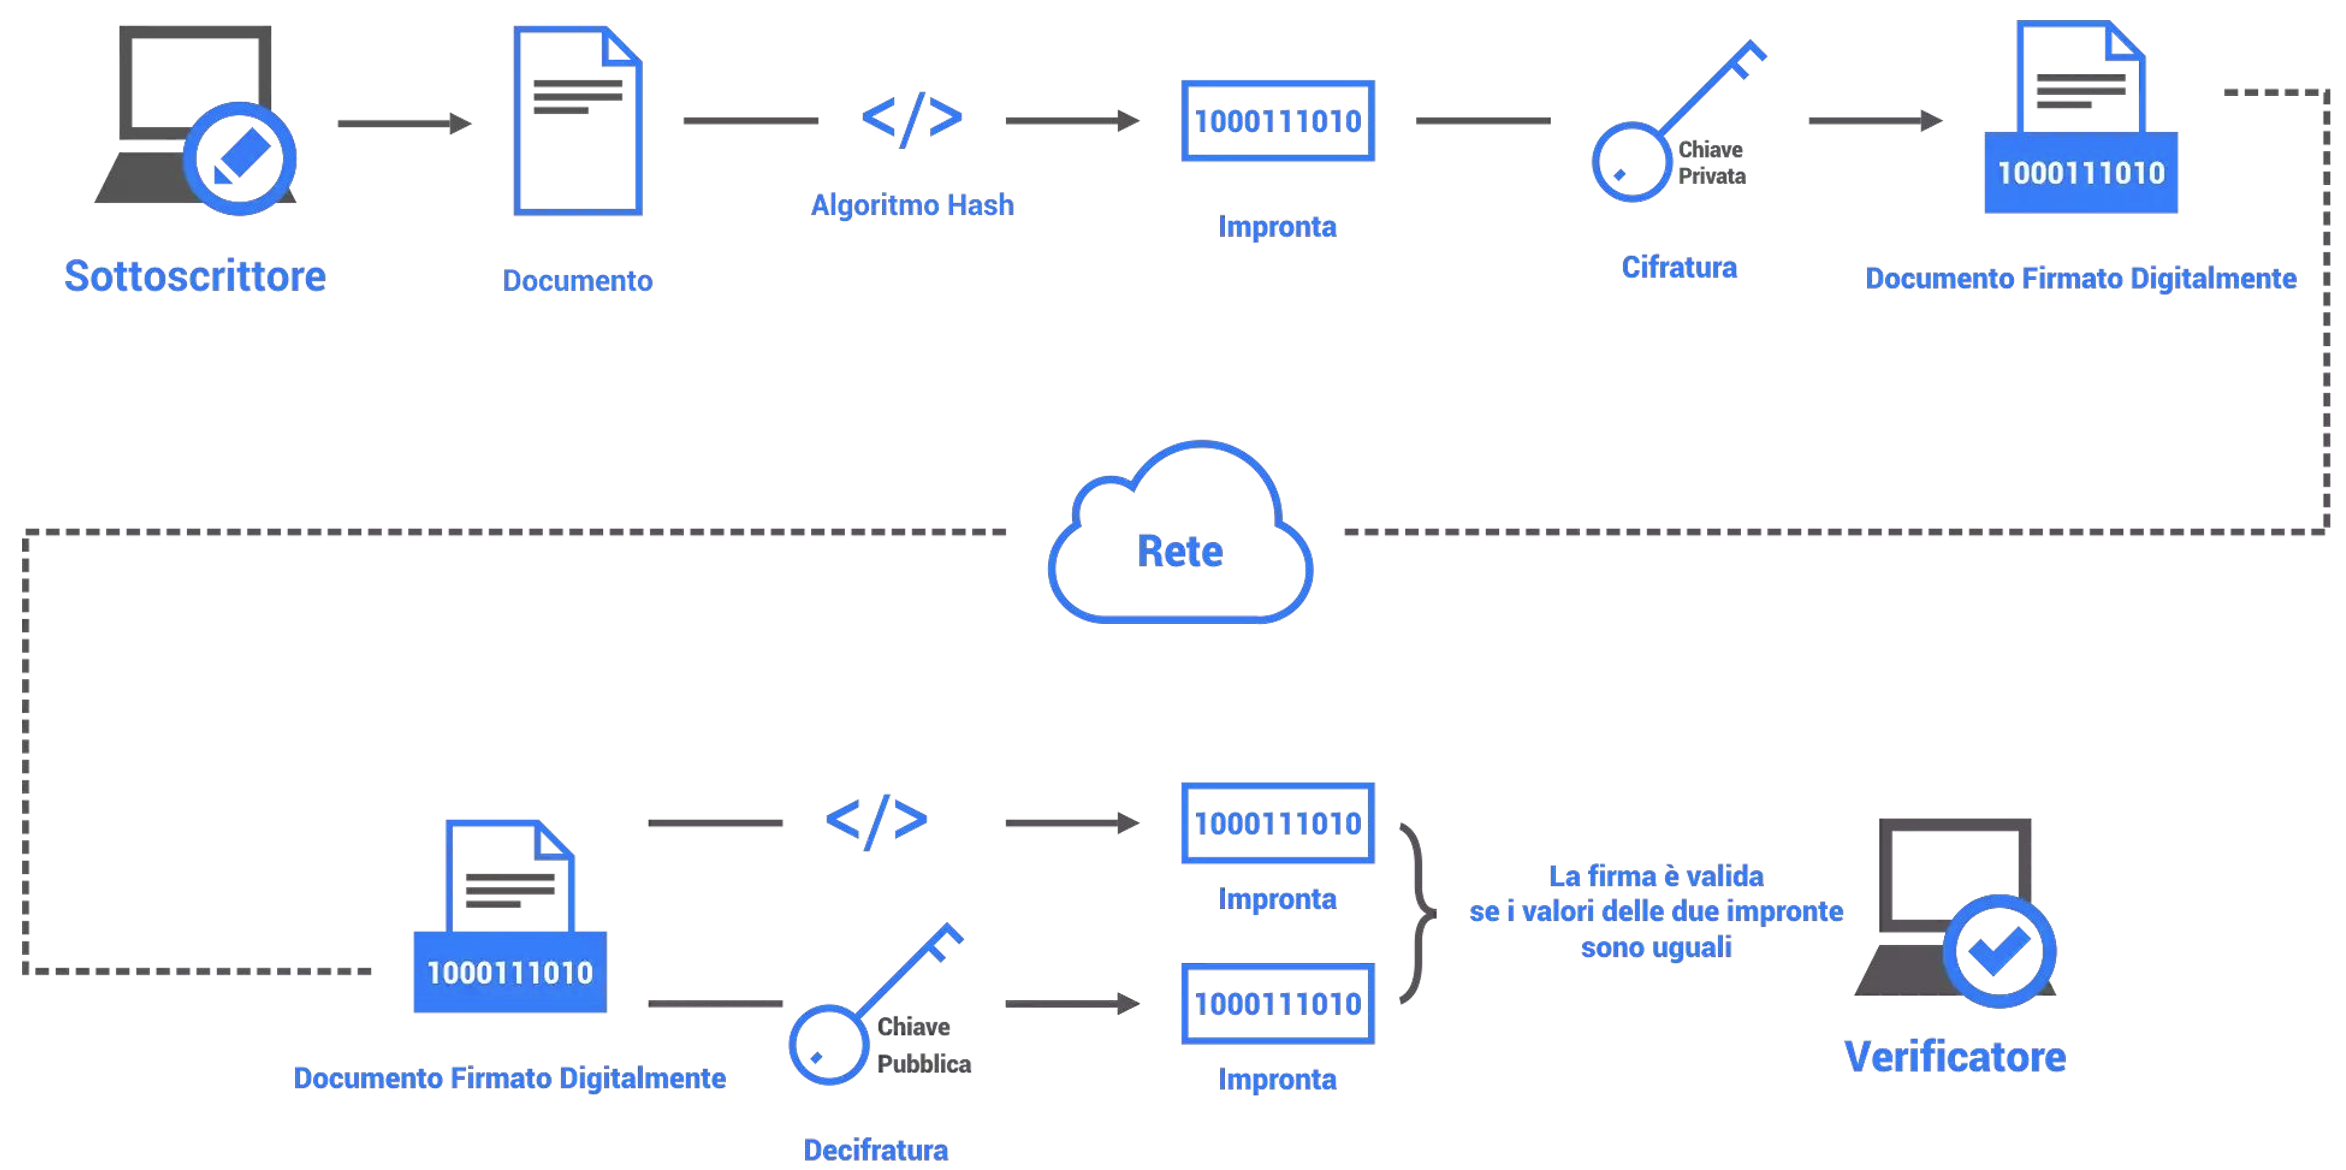
\includegraphics[width=\textwidth]{images/digital_sign.png}
                \caption{Digital signature schematics.}
                \label{fig:digital_sign}
            \end{center}
        \end{figure}
    \end{itemize}

\end{itemize}

\subsection{What Is a VPN?}

A VPN, or Virtual Private Network, is a technology that creates a secure connection over the internet between your device and a remote server or between two devices.

\subsubsection{Main Functions of a VPN}

\begin{itemize}
    \item \textbf{Security}: Encrypts traffic between your device and the VPN server, ensuring intercepted data cannot be read or interpreted.
    \item \textbf{Privacy}: Hides your real IP address and geographic location, making it difficult for websites and online services to track your activity or location.
    \item \textbf{Access to Geo-Blocked Resources}: Allows you to choose a VPN server, enabling you to bypass geographic restrictions.
    \item \textbf{Public Network Security}: Protects you from potential attacks when connected to public Wi-Fi networks, such as in cafes or airports.
\end{itemize}


\section{Python for Hackers and Web Applications}

\section{BUILD WEEK 1: Network Security design}
